% Options for packages loaded elsewhere
\PassOptionsToPackage{unicode}{hyperref}
\PassOptionsToPackage{hyphens}{url}
\PassOptionsToPackage{dvipsnames,svgnames,x11names}{xcolor}
%
\documentclass[
  letterpaper,
]{krantz}

\usepackage{amsmath,amssymb}
\usepackage{iftex}
\ifPDFTeX
  \usepackage[T1]{fontenc}
  \usepackage[utf8]{inputenc}
  \usepackage{textcomp} % provide euro and other symbols
\else % if luatex or xetex
  \usepackage{unicode-math}
  \defaultfontfeatures{Scale=MatchLowercase}
  \defaultfontfeatures[\rmfamily]{Ligatures=TeX,Scale=1}
\fi
\usepackage{lmodern}
\ifPDFTeX\else  
    % xetex/luatex font selection
\fi
% Use upquote if available, for straight quotes in verbatim environments
\IfFileExists{upquote.sty}{\usepackage{upquote}}{}
\IfFileExists{microtype.sty}{% use microtype if available
  \usepackage[]{microtype}
  \UseMicrotypeSet[protrusion]{basicmath} % disable protrusion for tt fonts
}{}
\makeatletter
\@ifundefined{KOMAClassName}{% if non-KOMA class
  \IfFileExists{parskip.sty}{%
    \usepackage{parskip}
  }{% else
    \setlength{\parindent}{0pt}
    \setlength{\parskip}{6pt plus 2pt minus 1pt}}
}{% if KOMA class
  \KOMAoptions{parskip=half}}
\makeatother
\usepackage{xcolor}
\setlength{\emergencystretch}{3em} % prevent overfull lines
\setcounter{secnumdepth}{5}
% Make \paragraph and \subparagraph free-standing
\ifx\paragraph\undefined\else
  \let\oldparagraph\paragraph
  \renewcommand{\paragraph}[1]{\oldparagraph{#1}\mbox{}}
\fi
\ifx\subparagraph\undefined\else
  \let\oldsubparagraph\subparagraph
  \renewcommand{\subparagraph}[1]{\oldsubparagraph{#1}\mbox{}}
\fi

\usepackage{color}
\usepackage{fancyvrb}
\newcommand{\VerbBar}{|}
\newcommand{\VERB}{\Verb[commandchars=\\\{\}]}
\DefineVerbatimEnvironment{Highlighting}{Verbatim}{commandchars=\\\{\}}
% Add ',fontsize=\small' for more characters per line
\usepackage{framed}
\definecolor{shadecolor}{RGB}{241,243,245}
\newenvironment{Shaded}{\begin{snugshade}}{\end{snugshade}}
\newcommand{\AlertTok}[1]{\textcolor[rgb]{0.68,0.00,0.00}{#1}}
\newcommand{\AnnotationTok}[1]{\textcolor[rgb]{0.37,0.37,0.37}{#1}}
\newcommand{\AttributeTok}[1]{\textcolor[rgb]{0.40,0.45,0.13}{#1}}
\newcommand{\BaseNTok}[1]{\textcolor[rgb]{0.68,0.00,0.00}{#1}}
\newcommand{\BuiltInTok}[1]{\textcolor[rgb]{0.00,0.23,0.31}{#1}}
\newcommand{\CharTok}[1]{\textcolor[rgb]{0.13,0.47,0.30}{#1}}
\newcommand{\CommentTok}[1]{\textcolor[rgb]{0.37,0.37,0.37}{#1}}
\newcommand{\CommentVarTok}[1]{\textcolor[rgb]{0.37,0.37,0.37}{\textit{#1}}}
\newcommand{\ConstantTok}[1]{\textcolor[rgb]{0.56,0.35,0.01}{#1}}
\newcommand{\ControlFlowTok}[1]{\textcolor[rgb]{0.00,0.23,0.31}{#1}}
\newcommand{\DataTypeTok}[1]{\textcolor[rgb]{0.68,0.00,0.00}{#1}}
\newcommand{\DecValTok}[1]{\textcolor[rgb]{0.68,0.00,0.00}{#1}}
\newcommand{\DocumentationTok}[1]{\textcolor[rgb]{0.37,0.37,0.37}{\textit{#1}}}
\newcommand{\ErrorTok}[1]{\textcolor[rgb]{0.68,0.00,0.00}{#1}}
\newcommand{\ExtensionTok}[1]{\textcolor[rgb]{0.00,0.23,0.31}{#1}}
\newcommand{\FloatTok}[1]{\textcolor[rgb]{0.68,0.00,0.00}{#1}}
\newcommand{\FunctionTok}[1]{\textcolor[rgb]{0.28,0.35,0.67}{#1}}
\newcommand{\ImportTok}[1]{\textcolor[rgb]{0.00,0.46,0.62}{#1}}
\newcommand{\InformationTok}[1]{\textcolor[rgb]{0.37,0.37,0.37}{#1}}
\newcommand{\KeywordTok}[1]{\textcolor[rgb]{0.00,0.23,0.31}{#1}}
\newcommand{\NormalTok}[1]{\textcolor[rgb]{0.00,0.23,0.31}{#1}}
\newcommand{\OperatorTok}[1]{\textcolor[rgb]{0.37,0.37,0.37}{#1}}
\newcommand{\OtherTok}[1]{\textcolor[rgb]{0.00,0.23,0.31}{#1}}
\newcommand{\PreprocessorTok}[1]{\textcolor[rgb]{0.68,0.00,0.00}{#1}}
\newcommand{\RegionMarkerTok}[1]{\textcolor[rgb]{0.00,0.23,0.31}{#1}}
\newcommand{\SpecialCharTok}[1]{\textcolor[rgb]{0.37,0.37,0.37}{#1}}
\newcommand{\SpecialStringTok}[1]{\textcolor[rgb]{0.13,0.47,0.30}{#1}}
\newcommand{\StringTok}[1]{\textcolor[rgb]{0.13,0.47,0.30}{#1}}
\newcommand{\VariableTok}[1]{\textcolor[rgb]{0.07,0.07,0.07}{#1}}
\newcommand{\VerbatimStringTok}[1]{\textcolor[rgb]{0.13,0.47,0.30}{#1}}
\newcommand{\WarningTok}[1]{\textcolor[rgb]{0.37,0.37,0.37}{\textit{#1}}}

\providecommand{\tightlist}{%
  \setlength{\itemsep}{0pt}\setlength{\parskip}{0pt}}\usepackage{longtable,booktabs,array}
\usepackage{calc} % for calculating minipage widths
% Correct order of tables after \paragraph or \subparagraph
\usepackage{etoolbox}
\makeatletter
\patchcmd\longtable{\par}{\if@noskipsec\mbox{}\fi\par}{}{}
\makeatother
% Allow footnotes in longtable head/foot
\IfFileExists{footnotehyper.sty}{\usepackage{footnotehyper}}{\usepackage{footnote}}
\makesavenoteenv{longtable}
\usepackage{graphicx}
\makeatletter
\def\maxwidth{\ifdim\Gin@nat@width>\linewidth\linewidth\else\Gin@nat@width\fi}
\def\maxheight{\ifdim\Gin@nat@height>\textheight\textheight\else\Gin@nat@height\fi}
\makeatother
% Scale images if necessary, so that they will not overflow the page
% margins by default, and it is still possible to overwrite the defaults
% using explicit options in \includegraphics[width, height, ...]{}
\setkeys{Gin}{width=\maxwidth,height=\maxheight,keepaspectratio}
% Set default figure placement to htbp
\makeatletter
\def\fps@figure{htbp}
\makeatother

\usepackage{booktabs}
\usepackage{longtable}
\usepackage[bf,singlelinecheck=off]{caption}
\usepackage[scale=.8]{sourcecodepro}
\usepackage{hyperref}

\usepackage{framed,color}
\definecolor{shadecolor}{RGB}{248,248,248}

\renewcommand{\textfraction}{0.05}
\renewcommand{\topfraction}{0.8}
\renewcommand{\bottomfraction}{0.8}
\renewcommand{\floatpagefraction}{0.75}

\renewenvironment{quote}{\begin{VF}}{\end{VF}}
\let\oldhref\href
\renewcommand{\href}[2]{#2\footnote{\url{#1}}}

\makeatletter
\newenvironment{kframe}{%
\medskip{}
\setlength{\fboxsep}{.8em}
 \def\at@end@of@kframe{}%
 \ifinner\ifhmode%
  \def\at@end@of@kframe{\end{minipage}}%
  \begin{minipage}{\columnwidth}%
 \fi\fi%
 \def\FrameCommand##1{\hskip\@totalleftmargin \hskip-\fboxsep
 \colorbox{shadecolor}{##1}\hskip-\fboxsep
     % There is no \\@totalrightmargin, so:
     \hskip-\linewidth \hskip-\@totalleftmargin \hskip\columnwidth}%
 \MakeFramed {\advance\hsize-\width
   \@totalleftmargin\z@ \linewidth\hsize
   \@setminipage}}%
 {\par\unskip\endMakeFramed%
 \at@end@of@kframe}
\makeatother

\renewenvironment{Shaded}{\begin{kframe}}{\end{kframe}}

\usepackage{makeidx}
\makeindex

\urlstyle{tt}

\usepackage{amsthm}
\makeatletter
\def\thm@space@setup{%
  \thm@preskip=8pt plus 2pt minus 4pt
  \thm@postskip=\thm@preskip
}
\makeatother

\frontmatter
\makeatletter
\makeatother
\makeatletter
\@ifpackageloaded{bookmark}{}{\usepackage{bookmark}}
\makeatother
\makeatletter
\@ifpackageloaded{caption}{}{\usepackage{caption}}
\AtBeginDocument{%
\ifdefined\contentsname
  \renewcommand*\contentsname{Table of contents}
\else
  \newcommand\contentsname{Table of contents}
\fi
\ifdefined\listfigurename
  \renewcommand*\listfigurename{List of Figures}
\else
  \newcommand\listfigurename{List of Figures}
\fi
\ifdefined\listtablename
  \renewcommand*\listtablename{List of Tables}
\else
  \newcommand\listtablename{List of Tables}
\fi
\ifdefined\figurename
  \renewcommand*\figurename{Figure}
\else
  \newcommand\figurename{Figure}
\fi
\ifdefined\tablename
  \renewcommand*\tablename{Table}
\else
  \newcommand\tablename{Table}
\fi
}
\@ifpackageloaded{float}{}{\usepackage{float}}
\floatstyle{ruled}
\@ifundefined{c@chapter}{\newfloat{codelisting}{h}{lop}}{\newfloat{codelisting}{h}{lop}[chapter]}
\floatname{codelisting}{Listing}
\newcommand*\listoflistings{\listof{codelisting}{List of Listings}}
\makeatother
\makeatletter
\@ifpackageloaded{caption}{}{\usepackage{caption}}
\@ifpackageloaded{subcaption}{}{\usepackage{subcaption}}
\makeatother
\makeatletter
\@ifpackageloaded{tcolorbox}{}{\usepackage[skins,breakable]{tcolorbox}}
\makeatother
\makeatletter
\@ifundefined{shadecolor}{\definecolor{shadecolor}{rgb}{.97, .97, .97}}
\makeatother
\makeatletter
\makeatother
\makeatletter
\makeatother
\ifLuaTeX
  \usepackage{selnolig}  % disable illegal ligatures
\fi
\IfFileExists{bookmark.sty}{\usepackage{bookmark}}{\usepackage{hyperref}}
\IfFileExists{xurl.sty}{\usepackage{xurl}}{} % add URL line breaks if available
\urlstyle{same} % disable monospaced font for URLs
\hypersetup{
  pdftitle={Proyek Sain Data},
  pdfauthor={Naufal Abdullah R.Z},
  colorlinks=true,
  linkcolor={blue},
  filecolor={Maroon},
  citecolor={Blue},
  urlcolor={Blue},
  pdfcreator={LaTeX via pandoc}}

\title{Proyek Sain Data}
\author{Naufal Abdullah R.Z}
\date{2023-12-04}

\begin{document}
\maketitle
% you may need to leave a few empty pages before the dedication page

%\cleardoublepage\newpage\thispagestyle{empty}\null
%\cleardoublepage\newpage\thispagestyle{empty}\null
%\cleardoublepage\newpage
\thispagestyle{empty}

\begin{center}
To blah, blah, and blah.
%\includegraphics{images/dedication.pdf}
\end{center}

\setlength{\abovedisplayskip}{-5pt}
\setlength{\abovedisplayshortskip}{-5pt}

\ifdefined\Shaded\renewenvironment{Shaded}{\begin{tcolorbox}[interior hidden, borderline west={3pt}{0pt}{shadecolor}, sharp corners, frame hidden, breakable, boxrule=0pt, enhanced]}{\end{tcolorbox}}\fi

\renewcommand*\contentsname{Table of contents}
{
\hypersetup{linkcolor=}
\setcounter{tocdepth}{2}
\tableofcontents
}
\bookmarksetup{startatroot}

\hypertarget{streamlit}{%
\chapter*{Streamlit}\label{streamlit}}
\addcontentsline{toc}{chapter}{Streamlit}

\markboth{Streamlit}{Streamlit}

link streamlit Dry Bean Streamlit

\mainmatter

\bookmarksetup{startatroot}

\hypertarget{dry-bean}{%
\chapter{Dry Bean}\label{dry-bean}}

Nama : Naufal Abdullah Rasyiq Zaki

NIM : 200411100096

\hypertarget{business-understanding}{%
\section{Business Understanding}\label{business-understanding}}

Tujuan utama dari proyek ini adalah mengembangkan model klasifikasi
untuk mengidentifikasi kategori biji-bijian kering berdasarkan fitur
yang ada. Hasilnya akan digunakan seperti:

\begin{itemize}
\tightlist
\item
  Membantu untuk mengklasifikasikan biji-bijian kering dari tujuh jenis
  kacang yang terdaftar berdasarkan fitur-fitur tertentu.
\item
  menyediakan alat identifikasi biji-bijian kering sesuai klasifikasi
  nya
\end{itemize}

\hypertarget{data-understanding}{%
\section{Data Understanding}\label{data-understanding}}

Dataset yang digunakan adalah data Dry Bean yang berasal dari website
UCI Machine Learning. Data ini merupakan sebuah dataset kumpulan gambar
biji-bijian dari tujuh jenis kacang yang berbeda menggunakan kamera
resolusi tinggi. Dataset yang digunakan memiliki 13611 data.

\hypertarget{penjelasan-atribut}{%
\subsection{Penjelasan atribut}\label{penjelasan-atribut}}

Berikut ini adalah penjelasan atribut atribut yang digunakan:

\begin{enumerate}
\def\labelenumi{\arabic{enumi}.}
\tightlist
\item
  Area (A) : Luas zona kacang dan jumlah piksel dalam batasnya.
\item
  Perimeter (P) : Keliling kacang didefinisikan sebagai panjang tepinya.
\item
  Major axis length (L) : Jarak antara ujung-ujung garis terpanjang yang
  dapat ditarik dari sebuah kacang.
\item
  Minor axis length (l) : Garis terpanjang yang dapat ditarik dari
  kacang sambil berdiri tegak lurus terhadap sumbu utama.
\item
  Aspect ratio (K) : Mendefinisikan hubungan antara L dan l.
\item
  Eccentricity (Ec) : Eksentrisitas elips yang momennya sama dengan
  daerah.
\item
  Convex area (C) : Jumlah piksel dalam poligon cembung terkecil yang
  dapat memuat luas biji kacang.
\item
  Equivalent diameter (Ed) : Diameter lingkaran yang luasnya sama dengan
  luas biji kacang.
\item
  Extent (Ex) : Rasio piksel dalam kotak pembatas dengan area kacang.
\item
  Solidity (S) : Juga dikenal sebagai konveksitas. Rasio piksel pada
  cangkang cembung dengan piksel pada kacang.
\item
  Roundness (R): Dihitung dengan rumus berikut: (4piA)/(P\^{}2)
\item
  Compactness (CO) : Mengukur kebulatan suatu benda: Ed/L
\item
  ShapeFactor1 (SF1) : Faktor Bentuk 1
\item
  ShapeFactor2 (SF2) : Faktor Bentuk 2
\item
  ShapeFactor3 (SF3) : Faktor Bentuk 3
\item
  ShapeFactor4 (SF4) : Faktor Bentuk 4
\item
  class (Seker, Barbunya, Bombay, Cali, Dermosan, Horoz and Sira)
\end{enumerate}

\hypertarget{library}{%
\subsection{Library}\label{library}}

\begin{Shaded}
\begin{Highlighting}[]
\ImportTok{import}\NormalTok{ matplotlib.pyplot }\ImportTok{as}\NormalTok{ plt}
\ImportTok{import}\NormalTok{ pandas }\ImportTok{as}\NormalTok{ pd}
\ImportTok{import}\NormalTok{ seaborn }\ImportTok{as}\NormalTok{ sns}
\ImportTok{import}\NormalTok{ numpy }\ImportTok{as}\NormalTok{ np}
\ImportTok{from}\NormalTok{ sklearn.feature\_selection }\ImportTok{import}\NormalTok{ SelectKBest, f\_classif}
\ImportTok{from}\NormalTok{ sklearn.preprocessing }\ImportTok{import}\NormalTok{ MinMaxScaler}

\end{Highlighting}
\end{Shaded}

\hypertarget{install-dataset-dry-bean}{%
\subsection{Install dataset dry bean}\label{install-dataset-dry-bean}}

\begin{Shaded}
\begin{Highlighting}[]
\ImportTok{from}\NormalTok{ google.colab }\ImportTok{import}\NormalTok{ drive}
\NormalTok{drive.mount(}\StringTok{\textquotesingle{}/content/drive\textquotesingle{}}\NormalTok{)}
\end{Highlighting}
\end{Shaded}

\begin{verbatim}
Drive already mounted at /content/drive; to attempt to forcibly remount, call drive.mount("/content/drive", force_remount=True).
\end{verbatim}

\begin{Shaded}
\begin{Highlighting}[]
\ImportTok{import}\NormalTok{ pandas }\ImportTok{as}\NormalTok{ pd}

\CommentTok{\# Memuat file CSV}
\NormalTok{df }\OperatorTok{=}\NormalTok{ pd.read\_excel(}\StringTok{\textquotesingle{}/content/drive/MyDrive/Proyek\_Sain\_Data/dry+bean+dataset/DryBeanDataset/Dry\_Bean\_Dataset.xlsx\textquotesingle{}}\NormalTok{)}

\CommentTok{\# Menampilkan tabel}
\NormalTok{df}
\end{Highlighting}
\end{Shaded}

\begin{longtable}[]{@{}llllllllllllllllll@{}}
\toprule\noalign{}
& Area & Perimeter & MajorAxisLength & MinorAxisLength & AspectRation &
Eccentricity & ConvexArea & EquivDiameter & Extent & Solidity &
roundness & Compactness & ShapeFactor1 & ShapeFactor2 & ShapeFactor3 &
ShapeFactor4 & Class \\
\midrule\noalign{}
\endhead
\bottomrule\noalign{}
\endlastfoot
0 & 28395 & 610.291 & 208.178117 & 173.888747 & 1.197191 & 0.549812 &
28715 & 190.141097 & 0.763923 & 0.988856 & 0.958027 & 0.913358 &
0.007332 & 0.003147 & 0.834222 & 0.998724 & SEKER \\
1 & 28734 & 638.018 & 200.524796 & 182.734419 & 1.097356 & 0.411785 &
29172 & 191.272750 & 0.783968 & 0.984986 & 0.887034 & 0.953861 &
0.006979 & 0.003564 & 0.909851 & 0.998430 & SEKER \\
2 & 29380 & 624.110 & 212.826130 & 175.931143 & 1.209713 & 0.562727 &
29690 & 193.410904 & 0.778113 & 0.989559 & 0.947849 & 0.908774 &
0.007244 & 0.003048 & 0.825871 & 0.999066 & SEKER \\
3 & 30008 & 645.884 & 210.557999 & 182.516516 & 1.153638 & 0.498616 &
30724 & 195.467062 & 0.782681 & 0.976696 & 0.903936 & 0.928329 &
0.007017 & 0.003215 & 0.861794 & 0.994199 & SEKER \\
4 & 30140 & 620.134 & 201.847882 & 190.279279 & 1.060798 & 0.333680 &
30417 & 195.896503 & 0.773098 & 0.990893 & 0.984877 & 0.970516 &
0.006697 & 0.003665 & 0.941900 & 0.999166 & SEKER \\
... & ... & ... & ... & ... & ... & ... & ... & ... & ... & ... & ... &
... & ... & ... & ... & ... & ... \\
13606 & 42097 & 759.696 & 288.721612 & 185.944705 & 1.552728 & 0.765002
& 42508 & 231.515799 & 0.714574 & 0.990331 & 0.916603 & 0.801865 &
0.006858 & 0.001749 & 0.642988 & 0.998385 & DERMASON \\
13607 & 42101 & 757.499 & 281.576392 & 190.713136 & 1.476439 & 0.735702
& 42494 & 231.526798 & 0.799943 & 0.990752 & 0.922015 & 0.822252 &
0.006688 & 0.001886 & 0.676099 & 0.998219 & DERMASON \\
13608 & 42139 & 759.321 & 281.539928 & 191.187979 & 1.472582 & 0.734065
& 42569 & 231.631261 & 0.729932 & 0.989899 & 0.918424 & 0.822730 &
0.006681 & 0.001888 & 0.676884 & 0.996767 & DERMASON \\
13609 & 42147 & 763.779 & 283.382636 & 190.275731 & 1.489326 & 0.741055
& 42667 & 231.653248 & 0.705389 & 0.987813 & 0.907906 & 0.817457 &
0.006724 & 0.001852 & 0.668237 & 0.995222 & DERMASON \\
13610 & 42159 & 772.237 & 295.142741 & 182.204716 & 1.619841 & 0.786693
& 42600 & 231.686223 & 0.788962 & 0.989648 & 0.888380 & 0.784997 &
0.007001 & 0.001640 & 0.616221 & 0.998180 & DERMASON \\
\end{longtable}

\begin{Shaded}
\begin{Highlighting}[]
\NormalTok{X }\OperatorTok{=}\NormalTok{ df.drop([}\StringTok{\textquotesingle{}Class\textquotesingle{}}\NormalTok{], axis}\OperatorTok{=}\DecValTok{1}\NormalTok{)}
\NormalTok{y }\OperatorTok{=}\NormalTok{ df[}\StringTok{"Class"}\NormalTok{]}
\end{Highlighting}
\end{Shaded}

\hypertarget{missing-value}{%
\subsection{Missing value}\label{missing-value}}

Cek apakah ada missing value pada dataset

\begin{Shaded}
\begin{Highlighting}[]
\BuiltInTok{print}\NormalTok{(X.isnull().}\BuiltInTok{sum}\NormalTok{())  }\CommentTok{\# Menampilkan jumlah missing value untuk setiap kolom}
\end{Highlighting}
\end{Shaded}

\begin{verbatim}
Area               0
Perimeter          0
MajorAxisLength    0
MinorAxisLength    0
AspectRation       0
Eccentricity       0
ConvexArea         0
EquivDiameter      0
Extent             0
Solidity           0
roundness          0
Compactness        0
ShapeFactor1       0
ShapeFactor2       0
ShapeFactor3       0
ShapeFactor4       0
dtype: int64
\end{verbatim}

\hypertarget{visualisasi}{%
\subsection{Visualisasi}\label{visualisasi}}

\begin{Shaded}
\begin{Highlighting}[]
\CommentTok{\# Menghitung jumlah biji kering dengan nilai biji tertentu}
\NormalTok{bean\_counts }\OperatorTok{=}\NormalTok{ y.value\_counts().sort\_index()}

\CommentTok{\# Membuat diagram garis untuk distribusi jumlah biji kering berdasarkan jumlah biji (bean)}
\NormalTok{plt.figure(figsize}\OperatorTok{=}\NormalTok{(}\DecValTok{8}\NormalTok{, }\DecValTok{6}\NormalTok{))}
\NormalTok{plt.plot(bean\_counts.index, bean\_counts.values, marker}\OperatorTok{=}\StringTok{\textquotesingle{}o\textquotesingle{}}\NormalTok{, color}\OperatorTok{=}\StringTok{\textquotesingle{}skyblue\textquotesingle{}}\NormalTok{, linestyle}\OperatorTok{=}\StringTok{\textquotesingle{}{-}\textquotesingle{}}\NormalTok{, linewidth}\OperatorTok{=}\DecValTok{2}\NormalTok{, markersize}\OperatorTok{=}\DecValTok{8}\NormalTok{)}
\NormalTok{plt.xlabel(}\StringTok{\textquotesingle{}Jumlah Kategori biji\textquotesingle{}}\NormalTok{)}
\NormalTok{plt.ylabel(}\StringTok{\textquotesingle{}Jumlah biji kering\textquotesingle{}}\NormalTok{)}
\NormalTok{plt.title(}\StringTok{\textquotesingle{}Distribusi Jumlah biji pada setiap kategori biji\textquotesingle{}}\NormalTok{)}
\NormalTok{plt.xticks(bean\_counts.index)}
\NormalTok{plt.grid(axis}\OperatorTok{=}\StringTok{\textquotesingle{}y\textquotesingle{}}\NormalTok{, linestyle}\OperatorTok{=}\StringTok{\textquotesingle{}{-}{-}\textquotesingle{}}\NormalTok{, alpha}\OperatorTok{=}\FloatTok{0.7}\NormalTok{)}

\CommentTok{\# Menambahkan label jumlah biji kering pada setiap titik pada diagram}
\ControlFlowTok{for}\NormalTok{ i, count }\KeywordTok{in} \BuiltInTok{enumerate}\NormalTok{(bean\_counts.values):}
\NormalTok{    plt.text(bean\_counts.index[i], count, }\BuiltInTok{str}\NormalTok{(count), ha}\OperatorTok{=}\StringTok{\textquotesingle{}center\textquotesingle{}}\NormalTok{, va}\OperatorTok{=}\StringTok{\textquotesingle{}bottom\textquotesingle{}}\NormalTok{)}

\NormalTok{plt.tight\_layout()}
\NormalTok{plt.show()}
\end{Highlighting}
\end{Shaded}

\begin{figure}[H]

{\centering 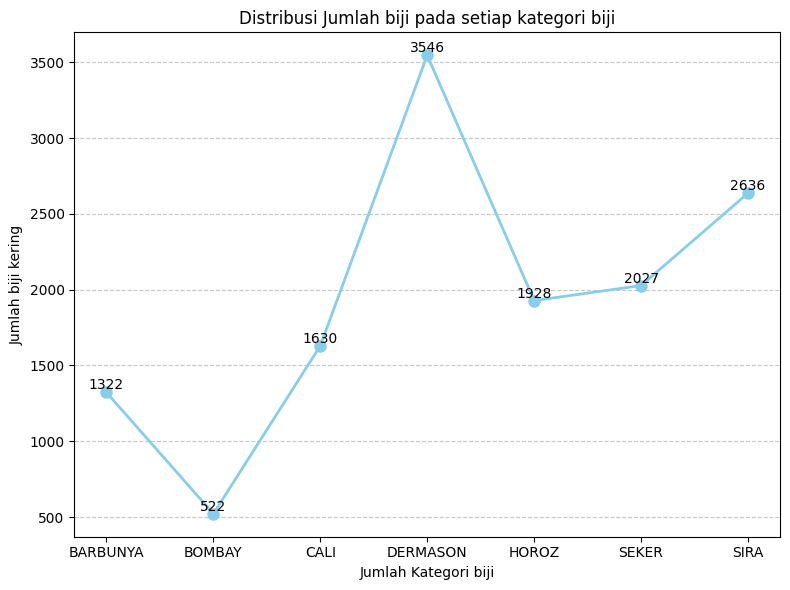
\includegraphics{Dry_Bean_20_096_files/figure-pdf/cell-7-output-1.png}

}

\end{figure}

Pada distribusi class ini, terlihat bahwa data dominan biji dermanson
berjumlah 3546 biji, sira berjumlah 2636, seker berjumlah 2027, horoz
berjumlah 1928, barbuya berjumlah 1322 dan data yang paling sedikit
yaitu biji bombay yang hanya berjumlah 522

\hypertarget{seleksi-fitur}{%
\subsection{Seleksi Fitur}\label{seleksi-fitur}}

sebelum melakukan preprocessing data alangkah baiknya untuk
menyeleksikan fitur fitur yang menurut kita adalah fitur yang tidak
berpengaruh terhadap dataset dan mengurangi beban dataset agar tidak
menyebabkan overfitting

Disini saya menggunakan sckit learn untuk melakukan selection pada fitur
- yang pertama saya menentukan banyaknya fitur terdapat N = banyak
fitur, fitur yang ada didataset adalah 16 fitur - Jumlah fitur terbaik
yang terpilih disesuaikan dengan nilai K di atas - ambil data data pada
setiap fitur menggunakan funtion colomns dan nama pada fitur akan
dimasukan kedalam selected\_feature\_names - lalu proses melakukan
perhitungan statistik ANOVA dengan rumus

\[
F = \frac{MSB}{MSW}
\] MSB atau mean square antar kelompok (mean square between groups).
dapat dari rumus ini :

\[
MSB = \frac{\sum_{i=1}^{k} n_i (\bar{X}_i - \bar{X}_{\text{total}})^2}{k - 1}
\] dan MSW atau mean square dalam kelompok (mean square within groups)

\[
MSW = \frac{\sum_{i=1}^{k} \sum_{j=1}^{n_i} (X_{ij} - \bar{X}_i)^2}{N - k}
\] Untuk hasil akhirnya saya menghapus 9 fitur yang menurut saya tidak
akan berpengaruh terhadap dataset

\begin{Shaded}
\begin{Highlighting}[]

\NormalTok{selector }\OperatorTok{=}\NormalTok{ SelectKBest(score\_func}\OperatorTok{=}\NormalTok{f\_classif, k}\OperatorTok{=}\DecValTok{15}\NormalTok{)  }\CommentTok{\# K adalah jumlah fitur terbaik yang akan dipilih}

\CommentTok{\# \# Lakukan seleksi fitur}
\NormalTok{selector.fit(X, y)}

\CommentTok{\# \# Tampilkan hasil seleksi fitur}
\CommentTok{\# \# Jumlah fitur terbaik yang terpilih disesuaikan dengan nilai K di atas}
\NormalTok{selected\_features }\OperatorTok{=}\NormalTok{ selector.get\_support(indices}\OperatorTok{=}\VariableTok{True}\NormalTok{)}
\NormalTok{feature\_names }\OperatorTok{=}\NormalTok{ X.columns}

\CommentTok{\# \#Pilih nama{-}nama fitur yang dipilih}
\NormalTok{selected\_feature\_names }\OperatorTok{=}\NormalTok{ [feature\_names[i] }\ControlFlowTok{for}\NormalTok{ i }\KeywordTok{in}\NormalTok{ selected\_features]}

\CommentTok{\# \# Sisa kode Anda tetap sama}
\CommentTok{\# \# Hitung skor statistik untuk setiap fitur}
\NormalTok{scores }\OperatorTok{=}\NormalTok{ selector.scores\_[selected\_features]}


\CommentTok{\# \# Membuat bar chart}
\NormalTok{plt.figure(figsize}\OperatorTok{=}\NormalTok{(}\DecValTok{10}\NormalTok{, }\DecValTok{6}\NormalTok{))}
\NormalTok{plt.bar(selected\_feature\_names, scores, color}\OperatorTok{=}\StringTok{\textquotesingle{}skyblue\textquotesingle{}}\NormalTok{)}
\NormalTok{plt.xlabel(}\StringTok{\textquotesingle{}Fitur\textquotesingle{}}\NormalTok{)}
\NormalTok{plt.ylabel(}\StringTok{\textquotesingle{}Skor Statistik\textquotesingle{}}\NormalTok{)}
\NormalTok{plt.title(}\StringTok{\textquotesingle{}Skor Statistik untuk Fitur{-}Fitur Terpilih\textquotesingle{}}\NormalTok{)}
\NormalTok{plt.xticks(rotation}\OperatorTok{=}\DecValTok{45}\NormalTok{)}
\NormalTok{plt.tight\_layout()}

\CommentTok{\# \# Menampilkan grafik}
\NormalTok{plt.show()}
\end{Highlighting}
\end{Shaded}

\begin{figure}[H]

{\centering 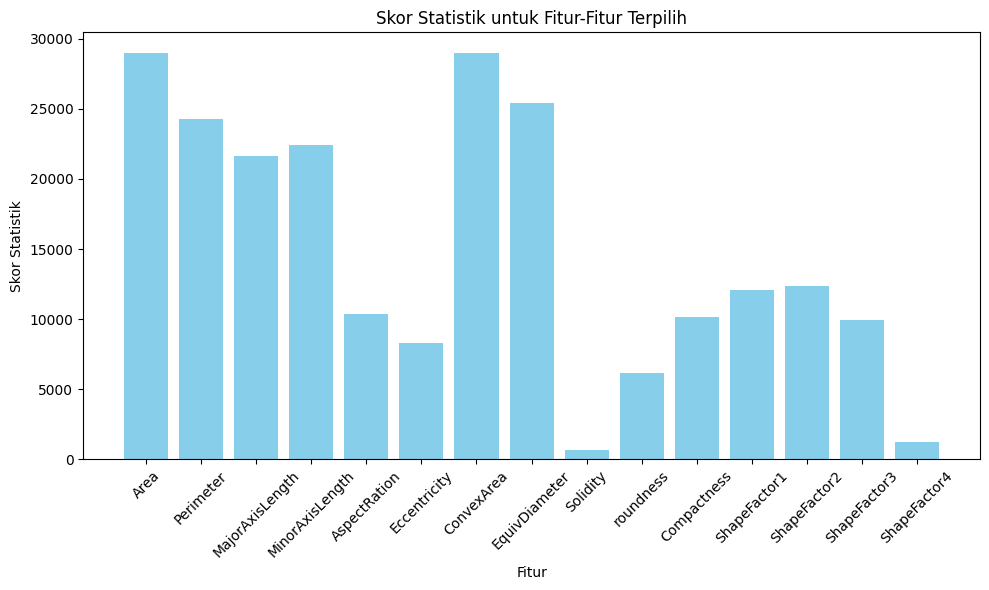
\includegraphics{Dry_Bean_20_096_files/figure-pdf/cell-8-output-1.png}

}

\end{figure}

\begin{Shaded}
\begin{Highlighting}[]
\NormalTok{X }\OperatorTok{=}\NormalTok{ df.drop([}\StringTok{\textquotesingle{}MinorAxisLength\textquotesingle{}}\NormalTok{,}\StringTok{\textquotesingle{}AspectRation\textquotesingle{}}\NormalTok{,}\StringTok{\textquotesingle{}Solidity\textquotesingle{}}\NormalTok{,}\StringTok{\textquotesingle{}roundness\textquotesingle{}}\NormalTok{,}\StringTok{\textquotesingle{}ShapeFactor4\textquotesingle{}}\NormalTok{,}\StringTok{\textquotesingle{}Class\textquotesingle{}}\NormalTok{], axis}\OperatorTok{=}\DecValTok{1}\NormalTok{)}
\NormalTok{X}
\end{Highlighting}
\end{Shaded}

\begin{longtable}[]{@{}llllllllllll@{}}
\toprule\noalign{}
& Area & Perimeter & MajorAxisLength & Eccentricity & ConvexArea &
EquivDiameter & Extent & Compactness & ShapeFactor1 & ShapeFactor2 &
ShapeFactor3 \\
\midrule\noalign{}
\endhead
\bottomrule\noalign{}
\endlastfoot
0 & 28395 & 610.291 & 208.178117 & 0.549812 & 28715 & 190.141097 &
0.763923 & 0.913358 & 0.007332 & 0.003147 & 0.834222 \\
1 & 28734 & 638.018 & 200.524796 & 0.411785 & 29172 & 191.272750 &
0.783968 & 0.953861 & 0.006979 & 0.003564 & 0.909851 \\
2 & 29380 & 624.110 & 212.826130 & 0.562727 & 29690 & 193.410904 &
0.778113 & 0.908774 & 0.007244 & 0.003048 & 0.825871 \\
3 & 30008 & 645.884 & 210.557999 & 0.498616 & 30724 & 195.467062 &
0.782681 & 0.928329 & 0.007017 & 0.003215 & 0.861794 \\
4 & 30140 & 620.134 & 201.847882 & 0.333680 & 30417 & 195.896503 &
0.773098 & 0.970516 & 0.006697 & 0.003665 & 0.941900 \\
... & ... & ... & ... & ... & ... & ... & ... & ... & ... & ... & ... \\
13606 & 42097 & 759.696 & 288.721612 & 0.765002 & 42508 & 231.515799 &
0.714574 & 0.801865 & 0.006858 & 0.001749 & 0.642988 \\
13607 & 42101 & 757.499 & 281.576392 & 0.735702 & 42494 & 231.526798 &
0.799943 & 0.822252 & 0.006688 & 0.001886 & 0.676099 \\
13608 & 42139 & 759.321 & 281.539928 & 0.734065 & 42569 & 231.631261 &
0.729932 & 0.822730 & 0.006681 & 0.001888 & 0.676884 \\
13609 & 42147 & 763.779 & 283.382636 & 0.741055 & 42667 & 231.653248 &
0.705389 & 0.817457 & 0.006724 & 0.001852 & 0.668237 \\
13610 & 42159 & 772.237 & 295.142741 & 0.786693 & 42600 & 231.686223 &
0.788962 & 0.784997 & 0.007001 & 0.001640 & 0.616221 \\
\end{longtable}

untuk membuang fitur yang skor statistik nya rendah

\hypertarget{preprocesing-data}{%
\section{Preprocesing Data}\label{preprocesing-data}}

\hypertarget{split-data}{%
\subsection{Split data}\label{split-data}}

train\_test\_split adalah suatu fungsi dalam library scikit-learn yang
digunakan untuk membagi dataset menjadi dua set, yaitu set pelatihan
(training set) dan set pengujian (testing set). Pemisahan ini bertujuan
untuk melakukan pelatihan model pada set pelatihan dan menguji kinerja
model pada set pengujian. Fungsi ini sangat umum digunakan dalam proses
machine learning untuk menghindari overfitting dan mengevaluasi
kemampuan generalisasi dari model yang telah dilatih

\begin{enumerate}
\def\labelenumi{\arabic{enumi}.}
\item
  test\_size (opsional): Menentukan ukuran set pengujian sebagai
  proporsi dari seluruh dataset. Nilai ini bisa berupa pecahan
  (misalnya, 0.2 untuk 20\%) atau bilangan bulat yang menyatakan jumlah
  sampel yang akan ditempatkan di set pengujian.
\item
  random\_state (opsional): Digunakan untuk mengontrol randomization
  selama pembagian dataset. Jika nilai ini diberikan, pemisahan dataset
  akan tetap konsisten setiap kali fungsi ini dijalankan
\end{enumerate}

\begin{Shaded}
\begin{Highlighting}[]
\ImportTok{from}\NormalTok{ sklearn.model\_selection }\ImportTok{import}\NormalTok{ train\_test\_split}


\CommentTok{\# Pembagian data menjadi data latih dan data uji (80\% data latih, 20\% data uji)}
\NormalTok{X\_train, X\_test, y\_train, y\_test }\OperatorTok{=}\NormalTok{ train\_test\_split(X, y, test\_size}\OperatorTok{=}\FloatTok{0.2}\NormalTok{, random\_state}\OperatorTok{=}\DecValTok{42}\NormalTok{)}
\end{Highlighting}
\end{Shaded}

\begin{Shaded}
\begin{Highlighting}[]
\NormalTok{X\_train.shape}
\end{Highlighting}
\end{Shaded}

\begin{verbatim}
(10888, 11)
\end{verbatim}

\begin{Shaded}
\begin{Highlighting}[]
\NormalTok{y\_train}
\end{Highlighting}
\end{Shaded}

\begin{verbatim}
11073    DERMASON
13172    DERMASON
11587    DERMASON
12492    DERMASON
430         SEKER
           ...   
5191         CALI
13418    DERMASON
5390         CALI
860         SEKER
7270        HOROZ
Name: Class, Length: 10888, dtype: object
\end{verbatim}

\hypertarget{normalisasi-data}{%
\subsection{Normalisasi Data}\label{normalisasi-data}}

Setelah melakukan understanding data maka melakukan preprocessing yang
dimana data akan di jadikan antara 0 sampai 1

dengan menggunakan minmaxScaller untuk menormalisasi data , dan
menggunakan train\_test\_split untuk mendapatkan data training dan data
testing

rumus MinmaxScaler:

\[
\text{Scaled Value} = \frac{\text{Original Value} - \text{Min}}{\text{Max} - \text{Min}}
\] - Original Value adalah nilai asli dari fitur.

\begin{itemize}
\item
  Min adalah nilai minimum dari fitur.
\item
  Max adalah nilai maksimum dari fitur.
\end{itemize}

\begin{enumerate}
\def\labelenumi{\arabic{enumi}.}
\item
  fit\_transform Fungsinya ini menghitung parameter normalisasi dari
  dataset (seperti nilai minimum dan maksimum) dan kemudian
  mengaplikasikan normalisasi pada dataset tersebut. Fungsi ini berguna
  untuk menghitung parameter normalisasi berdasarkan data pelatihan dan
  sekaligus menerapkan normalisasi tersebut.
\item
  Setelah kita telah menggunakan fit\_transform pada data pelatihan,
  kita dapat menggunakan metode transform pada data pengujian (dan data
  lainnya yang ingin dinormalisasi) menggunakan parameter normalisasi
  yang telah dihitung sebelumnya. Metode ini hanya melakukan normalisasi
  tanpa perlu menghitung parameter normalisasi lagi.
\end{enumerate}

\begin{Shaded}
\begin{Highlighting}[]
\NormalTok{scaler }\OperatorTok{=}\NormalTok{ MinMaxScaler()}
\NormalTok{X\_train\_scaler }\OperatorTok{=}\NormalTok{ scaler.fit\_transform(X\_train)}
\NormalTok{X\_test\_scaler }\OperatorTok{=}\NormalTok{ scaler.transform(X\_test)}
\NormalTok{x }\OperatorTok{=}\NormalTok{ pd.DataFrame(X\_train,columns}\OperatorTok{=}\NormalTok{X.columns)}
\NormalTok{x}
\end{Highlighting}
\end{Shaded}

\begin{longtable}[]{@{}llllllllllll@{}}
\toprule\noalign{}
& Area & Perimeter & MajorAxisLength & Eccentricity & ConvexArea &
EquivDiameter & Extent & Compactness & ShapeFactor1 & ShapeFactor2 &
ShapeFactor3 \\
\midrule\noalign{}
\endhead
\bottomrule\noalign{}
\endlastfoot
11073 & 29076 & 636.353 & 235.061516 & 0.740272 & 29490 & 192.407674 &
0.693524 & 0.818542 & 0.008084 & 0.002239 & 0.670011 \\
13172 & 38091 & 755.186 & 271.077683 & 0.748513 & 38716 & 220.224811 &
0.706318 & 0.812405 & 0.007117 & 0.001912 & 0.660002 \\
11587 & 30969 & 651.527 & 230.164083 & 0.664964 & 31318 & 198.572293 &
0.733689 & 0.862742 & 0.007432 & 0.002540 & 0.744324 \\
12492 & 34589 & 685.425 & 253.001232 & 0.723664 & 34965 & 209.857291 &
0.784331 & 0.829471 & 0.007314 & 0.002136 & 0.688023 \\
430 & 35954 & 710.093 & 251.660769 & 0.690581 & 36380 & 213.958067 &
0.794564 & 0.850184 & 0.007000 & 0.002256 & 0.722814 \\
... & ... & ... & ... & ... & ... & ... & ... & ... & ... & ... & ... \\
5191 & 83266 & 1117.778 & 448.473710 & 0.847920 & 84030 & 325.603384 &
0.797239 & 0.726026 & 0.005386 & 0.000923 & 0.527113 \\
13418 & 39857 & 755.392 & 283.623668 & 0.774448 & 40330 & 225.272077 &
0.692154 & 0.794264 & 0.007116 & 0.001747 & 0.630855 \\
5390 & 90004 & 1156.599 & 456.836383 & 0.833583 & 90790 & 338.521273 &
0.783939 & 0.741012 & 0.005076 & 0.000944 & 0.549099 \\
860 & 38426 & 711.412 & 246.696608 & 0.593467 & 38799 & 221.191100 &
0.752094 & 0.896612 & 0.006420 & 0.002559 & 0.803913 \\
7270 & 63628 & 997.390 & 400.784151 & 0.860715 & 64287 & 284.629032 &
0.622583 & 0.710180 & 0.006299 & 0.000988 & 0.504356 \\
\end{longtable}

\hypertarget{modelling}{%
\section{Modelling}\label{modelling}}

\hypertarget{random-forest}{%
\subsection{Random Forest}\label{random-forest}}

Rumus umum Random Forest
\[f(x) = \text{sign}\left(\frac{1}{N} \sum_{i=1}^{N} f_i(x) - \theta\right)
\] Dengan penjelasan:
\[\\\ N \text{ adalah jumlah pohon dalam hutan, } \\\ f_i(x) \text{ adalah prediksi dari pohon ke-} i,\\\ \text{ dan } \theta \text{ adalah ambang batas (threshold).}\]

\begin{Shaded}
\begin{Highlighting}[]
\ImportTok{from}\NormalTok{ sklearn.ensemble }\ImportTok{import}\NormalTok{ RandomForestClassifier}
\ImportTok{from}\NormalTok{ sklearn.metrics }\ImportTok{import}\NormalTok{ accuracy\_score, classification\_report}


\CommentTok{\#Buat model Random Forest}
\NormalTok{random\_forest\_model }\OperatorTok{=}\NormalTok{ RandomForestClassifier(n\_estimators}\OperatorTok{=}\DecValTok{100}\NormalTok{)}
\CommentTok{\#Latih model}
\NormalTok{random\_forest\_model.fit(X\_train, y\_train)}
\CommentTok{\#Prediksi dengan model}
\NormalTok{random\_forest\_predictions }\OperatorTok{=}\NormalTok{ random\_forest\_model.predict(X\_test)}
\CommentTok{\#Evaluasi kinerja model}
\NormalTok{random\_forest\_accuracy }\OperatorTok{=}\NormalTok{ accuracy\_score(y\_test, random\_forest\_predictions)}
\end{Highlighting}
\end{Shaded}

\hypertarget{decision-tree}{%
\subsection{Decision Tree}\label{decision-tree}}

Rumus umum Decision Tree: \[
f(x) = \text{sign}\left(\text{Node}(x) - \theta\right)
\] Dengan penjelasan: \[
\text{Node}(x):\text{Fungsi keputusan pohon keputusan untuk input } x
\\\ \theta: \text{ adalah ambang batas (threshold).}
\]

\begin{Shaded}
\begin{Highlighting}[]
\ImportTok{from}\NormalTok{ sklearn.tree }\ImportTok{import}\NormalTok{ DecisionTreeClassifier}
\ImportTok{from}\NormalTok{ sklearn.metrics }\ImportTok{import}\NormalTok{ accuracy\_score, classification\_report}

\NormalTok{decision\_tree\_model }\OperatorTok{=}\NormalTok{ DecisionTreeClassifier()}
\CommentTok{\#Latih model}
\NormalTok{decision\_tree\_model.fit(X\_train, y\_train)}
\CommentTok{\#Prediksi dengan model}
\NormalTok{decision\_tree\_predictions }\OperatorTok{=}\NormalTok{ decision\_tree\_model.predict(X\_test)}
\CommentTok{\#Evaluasi kinerja model}
\NormalTok{decision\_tree\_accuracy }\OperatorTok{=}\NormalTok{ accuracy\_score(y\_test, decision\_tree\_predictions)}
\end{Highlighting}
\end{Shaded}

\hypertarget{logistic-regresion}{%
\subsection{Logistic Regresion}\label{logistic-regresion}}

Rumus umum Logistic Regression: \[
f(x) = \frac{1}{1 + \exp(-\left(\sum_{i=1}^{N} w_i x_i + b\right))}
\] Dengan penjelasan: \[
\begin{align*}
f(x) & : \text{Fungsi keputusan Logistic Regression untuk input } x \\
w_i & : \text{Bobot input ke-} i \\
x_i & : \text{Input ke-} i \\
b & : \text{Bias}
\end{align*}
\]

\begin{Shaded}
\begin{Highlighting}[]
\ImportTok{from}\NormalTok{ sklearn.linear\_model }\ImportTok{import}\NormalTok{ LogisticRegression}
\ImportTok{from}\NormalTok{ sklearn.metrics }\ImportTok{import}\NormalTok{ accuracy\_score, classification\_report}

\NormalTok{model }\OperatorTok{=}\NormalTok{ LogisticRegression()}

\CommentTok{\#Latih model}
\NormalTok{model.fit(X\_train\_scaler, y\_train)}

\CommentTok{\#Prediksi dengan model}
\NormalTok{logistic\_regression\_predictions }\OperatorTok{=}\NormalTok{ model.predict(X\_test)}

\CommentTok{\#Evaluasi kinerja model}
\NormalTok{logistic\_regression\_accuracy }\OperatorTok{=}\NormalTok{ accuracy\_score(y\_test, logistic\_regression\_predictions)}
\end{Highlighting}
\end{Shaded}

\begin{verbatim}
/usr/local/lib/python3.10/dist-packages/sklearn/linear_model/_logistic.py:458: ConvergenceWarning: lbfgs failed to converge (status=1):
STOP: TOTAL NO. of ITERATIONS REACHED LIMIT.

Increase the number of iterations (max_iter) or scale the data as shown in:
    https://scikit-learn.org/stable/modules/preprocessing.html
Please also refer to the documentation for alternative solver options:
    https://scikit-learn.org/stable/modules/linear_model.html#logistic-regression
  n_iter_i = _check_optimize_result(
/usr/local/lib/python3.10/dist-packages/sklearn/base.py:432: UserWarning: X has feature names, but LogisticRegression was fitted without feature names
  warnings.warn(
\end{verbatim}

\hypertarget{neural-network}{%
\subsection{Neural Network}\label{neural-network}}

Rumus umum ANN: \[
f(x) = \text{sign}\left(\sum_{j=1}^{M} w_j g\left(\sum_{i=1}^{N} w_{ij} x_i + b_j\right) + b\right)
\] Dengan penjelasan: \[
\begin{align*}
f(x) & : \text{Fungsi keputusan ANN untuk input } x \\
w_j & : \text{Bobot output ke-} j \\
g(\cdot) & : \text{Fungsi aktivasi} \\
w_{ij} & : \text{Bobot input ke-} j \\
x_i & : \text{Input ke-} i \\
b_j & : \text{Bias ke-} j \\
b & : \text{Bias output}
\end{align*}
\]

\begin{Shaded}
\begin{Highlighting}[]
\ImportTok{from}\NormalTok{ sklearn.neural\_network }\ImportTok{import}\NormalTok{ MLPClassifier}
\ImportTok{from}\NormalTok{ sklearn.metrics }\ImportTok{import}\NormalTok{ accuracy\_score, classification\_report}

\CommentTok{\#Buat model Jaringan Saraf Tiruan}
\NormalTok{neural\_network\_model }\OperatorTok{=}\NormalTok{ MLPClassifier(hidden\_layer\_sizes}\OperatorTok{=}\NormalTok{(}\DecValTok{64}\NormalTok{, }\DecValTok{32}\NormalTok{), max\_iter}\OperatorTok{=}\DecValTok{1000}\NormalTok{, random\_state}\OperatorTok{=}\DecValTok{42}\NormalTok{)}

\CommentTok{\#Latih model}
\NormalTok{neural\_network\_model.fit(X\_train\_scaler, y\_train)}

\CommentTok{\#Prediksi dengan model}
\NormalTok{neural\_network\_predictions }\OperatorTok{=}\NormalTok{ neural\_network\_model.predict(X\_test)}

\CommentTok{\#Evaluasi kinerja model}
\NormalTok{neural\_network\_accuracy }\OperatorTok{=}\NormalTok{ accuracy\_score(y\_test, neural\_network\_predictions)}
\end{Highlighting}
\end{Shaded}

\begin{verbatim}
/usr/local/lib/python3.10/dist-packages/sklearn/base.py:432: UserWarning: X has feature names, but MLPClassifier was fitted without feature names
  warnings.warn(
\end{verbatim}

\hypertarget{evaluasi}{%
\section{Evaluasi}\label{evaluasi}}

Akurasi yang saya dapat adalah paling tinggi di model yang lain, maka
saya memilih metode random forest, alasan lainnya mengapa menggunakan
Random Forest Dengan mempertimbangkan akurasinya lebih tinggi dari pada
model yang lain.

\begin{Shaded}
\begin{Highlighting}[]
\BuiltInTok{print}\NormalTok{(}\StringTok{"Akurasi decision\_tree:"}\NormalTok{, decision\_tree\_accuracy)}
\BuiltInTok{print}\NormalTok{(}\StringTok{"Akurasi Random Forest:"}\NormalTok{, random\_forest\_accuracy)}
\BuiltInTok{print}\NormalTok{(}\StringTok{"Akurasi Regresi Logistik:"}\NormalTok{, logistic\_regression\_accuracy)}
\BuiltInTok{print}\NormalTok{(}\StringTok{"Akurasi neural\_network:"}\NormalTok{, neural\_network\_accuracy)}
\end{Highlighting}
\end{Shaded}

\begin{verbatim}
Akurasi decision_tree: 0.8788101358795446
Akurasi Random Forest: 0.9063532868160118
Akurasi Regresi Logistik: 0.04296731546088873
Akurasi neural_network: 0.04296731546088873
\end{verbatim}

\begin{Shaded}
\begin{Highlighting}[]
\ImportTok{import}\NormalTok{ matplotlib.pyplot }\ImportTok{as}\NormalTok{ plt}

\CommentTok{\# Data akurasi}
\NormalTok{models }\OperatorTok{=}\NormalTok{ [}\StringTok{\textquotesingle{}Decision Tree\textquotesingle{}}\NormalTok{, }\StringTok{\textquotesingle{}Random Forest\textquotesingle{}}\NormalTok{, }\StringTok{\textquotesingle{}Logistic Regression\textquotesingle{}}\NormalTok{, }\StringTok{\textquotesingle{}Neural Network\textquotesingle{}}\NormalTok{]}
\NormalTok{accuracies }\OperatorTok{=}\NormalTok{ [decision\_tree\_accuracy, random\_forest\_accuracy, logistic\_regression\_accuracy, neural\_network\_accuracy]}

\CommentTok{\# Membuat diagram batang}
\NormalTok{plt.figure(figsize}\OperatorTok{=}\NormalTok{(}\DecValTok{10}\NormalTok{, }\DecValTok{6}\NormalTok{))}
\NormalTok{plt.bar(models, accuracies, color}\OperatorTok{=}\NormalTok{[}\StringTok{\textquotesingle{}blue\textquotesingle{}}\NormalTok{, }\StringTok{\textquotesingle{}orange\textquotesingle{}}\NormalTok{, }\StringTok{\textquotesingle{}green\textquotesingle{}}\NormalTok{, }\StringTok{\textquotesingle{}purple\textquotesingle{}}\NormalTok{])}
\NormalTok{plt.ylim(}\DecValTok{0}\NormalTok{, }\DecValTok{1}\NormalTok{)  }\CommentTok{\# Menetapkan batas y{-}axis antara 0 dan 1}
\NormalTok{plt.title(}\StringTok{\textquotesingle{}Akurasi Model Klasifikasi\textquotesingle{}}\NormalTok{)}
\NormalTok{plt.xlabel(}\StringTok{\textquotesingle{}Model\textquotesingle{}}\NormalTok{)}
\NormalTok{plt.ylabel(}\StringTok{\textquotesingle{}Akurasi\textquotesingle{}}\NormalTok{)}
\NormalTok{plt.show()}
\end{Highlighting}
\end{Shaded}

\begin{figure}[H]

{\centering 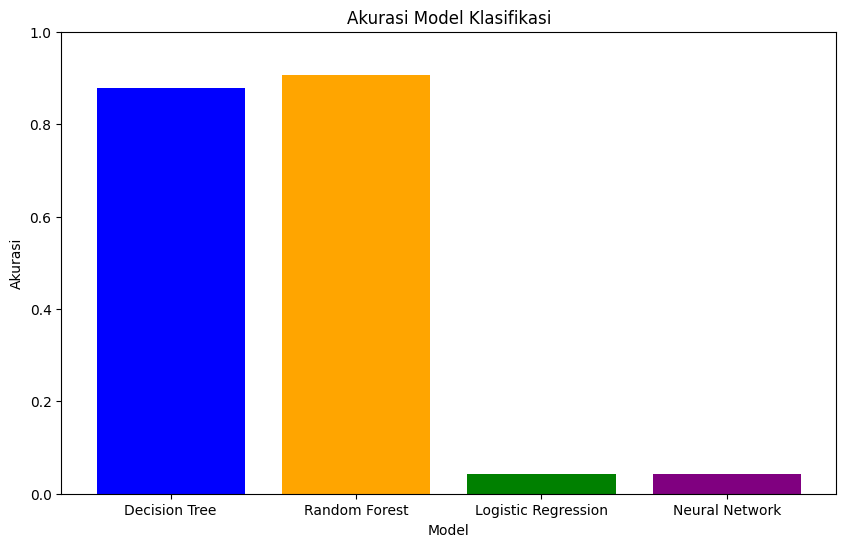
\includegraphics{Dry_Bean_20_096_files/figure-pdf/cell-20-output-1.png}

}

\end{figure}

Save Model

\begin{Shaded}
\begin{Highlighting}[]
\ImportTok{import}\NormalTok{ joblib}
\NormalTok{joblib.dump(random\_forest\_model, }\StringTok{\textquotesingle{}/content/drive/MyDrive/Proyek\_Sain\_Data/dry+bean+dataset/Model/saved\_data.joblib\textquotesingle{}}\NormalTok{)}
\end{Highlighting}
\end{Shaded}

\begin{verbatim}
['/content/drive/MyDrive/Proyek_Sain_Data/dry+bean+dataset/Model/saved_data.joblib']
\end{verbatim}



\backmatter
\printindex

\end{document}
